% Appendix is one-column so the wide dataset tables and the figure gallery have room.
\onecolumn

\chapter{The RBM-1M Dataset}
\label{apx:rbm1m}

RBM-1M is the corpus RoboRef re-curates, the training set behind Robometer \citep{robometer}. Table~\ref{tab:rbm1m} gives its composition from our scan of the released archives, one row per major source, grouped by embodiment. That grouping is the one that drives the re-curation. The standard robot arms are the manipulation data our work centers on, and they hold every failure in the corpus. The humanoid and human-only groups are large and broaden the visual coverage, but sit away from the single-arm setting our downstream tasks use, which is why we hold them out of the shared training corpus. A selection of them, listed in Appendix~\ref{apx:roboref-data}, is used once, in the first training phase of the Qwen3.5 model (Section~\ref{sec:method-dataset}).

\begin{table}[h]
\centering\footnotesize
\caption[Composition of RBM-1M]{Composition of RBM-1M, the corpus RoboRef re-curates, from a scan of Robometer's released archives. Sources are grouped by embodiment, and only the standard robot arms carry failures. Counts are archive-level entries, one row per camera view; the text explains why they run ahead of the number of distinct trajectories.}
\label{tab:rbm1m}
\begin{tabular}{@{}p{6.6cm}rrr@{}}
\toprule
Source & Failures & Successes & Total \\
\midrule
\multicolumn{4}{@{}l}{\emph{Humanoid}}\\
AgiBot \citep{agibot-world-contributors_agibot_2025} & 0 & 433{,}821 & 433{,}821 \\
Galaxea \citep{jiang_galaxea_2025} & 0 & 108{,}118 & 108{,}118 \\
Humanoid Everyday \citep{zhao_humanoid_2025} & 0 & 9{,}208 & 9{,}208 \\
\quad Subtotal & 0 & 551{,}147 & 551{,}147 \\
\addlinespace
\multicolumn{4}{@{}l}{\emph{Human-only (hand)}}\\
EgoDex \citep{hoque_egodex_2025} & 0 & 313{,}109 & 313{,}109 \\
EPIC \citep{damen_scaling_2018} & 0 & 37{,}030 & 37{,}030 \\
RH20T, human \citep{fang_rh20t_2024} & 0 & 14{,}225 & 14{,}225 \\
H2R & 0 & 2{,}254 & 2{,}254 \\
Other human-hand archives & 0 & 81 & 81 \\
\quad Subtotal & 0 & 366{,}699 & 366{,}699 \\
\addlinespace
\multicolumn{4}{@{}l}{\emph{Standard robot arms}}\\
DROID \citep{khazatsky_droid_2024} & 0 & 149{,}804 & 149{,}804 \\
RT-1 (Fractal) \citep{oneill_open_2024} & 0 & 87{,}204 & 87{,}204 \\
Bridge V2 \citep{oneill_open_2024} & 0 & 83{,}024 & 83{,}024 \\
Language Table \citep{oneill_open_2024} & 0 & 50{,}000 & 50{,}000 \\
BC-Z \citep{oneill_open_2024} & 0 & 43{,}261 & 43{,}261 \\
RoboSet \citep{oneill_open_2024} & 0 & 36{,}480 & 36{,}480 \\
RH20T \citep{fang_rh20t_2024} & 0 & 15{,}744 & 15{,}744 \\
MolmoAct \citep{lee_molmoact_2025} & 0 & 15{,}546 & 15{,}546 \\
FailSafe \citep{lin_failsafe_2025} & 58{,}153 & 13{,}461 & 71{,}614 \\
RoboReward \citep{roboreward} & 88{,}418 & 19{,}852 & 108{,}270 \\
RACER \citep{dai_racer_2025} & 29{,}211 & 7{,}131 & 36{,}342 \\
RoboArena \citep{atreya_roboarena_2025} & 17{,}510 & 2{,}635 & 20{,}145 \\
SOAR \citep{zhou_autonomous_2024} & 12{,}009 & 4{,}803 & 16{,}812 \\
LIBERO \citep{liu_libero_2023} & 6{,}241 & 5{,}659 & 11{,}900 \\
AutoEval \citep{zhou_autoeval_2025} & 3{,}721 & 4{,}956 & 8{,}677 \\
Furniture Bench \citep{heo_furniturebench_2023} & 0 & 5{,}100 & 5{,}100 \\
MetaWorld (ReWiND) \citep{zhang_rewind_2025} & 0 & 100 & 100 \\
Other standard-arm archives & 274 & 13{,}716 & 13{,}990 \\
\quad Subtotal & 215{,}537 & 558{,}476 & 774{,}013 \\
\midrule
Total & 215{,}537 & 1{,}476{,}322 & 1{,}691{,}859 \\
\bottomrule
\end{tabular}
\end{table}

The counts are archive-level entries, not distinct trajectories. Several sources are expanded across camera views, the long-horizon humanoid data across annotated sub-steps, and RoboReward is stored at two resolutions, so these figures run ahead of the number of unique recorded attempts. AgiBot is the clearest case of the first, about $34{,}000$ long-horizon trajectories appearing as $216{,}911$ sub-step entries under each of two camera archives, and the RoboReward archives hold every clip twice, once per resolution. This expansion, together with the re-curation of Section~\ref{sec:method-dataset}, is why RBM-1M counts well over a million entries here while our re-curated standard-arm corpus holds $648{,}714$ rows. The same two effects also explain why our per-source counts do not line up with Robometer's published Table~IX. We count one row per scored clip, an episode from a single camera view, while Robometer counts every unique video-language annotation expanded across views, so we report our own episode-level numbers throughout and do not attempt a row-by-row reconciliation. The 100 MetaWorld demonstrations listed are ReWiND's, the only MetaWorld in RBM-1M; our re-curation drops them in favor of the MetaWorld data we generate ourselves (Section~\ref{sec:method-dataset}).

\chapter{The RoboRef Dataset}
\label{apx:roboref-data}

This appendix expands the summary of Section~\ref{sec:method-dataset}. Table~\ref{tab:roboref-dataset} there reports the composition at the level the main text needs. Here we break the same corpus down to one row per upstream source, say where each failure label comes from, and give the pairing and sampling details the training pipeline relies on. Unless noted, every count below describes the standard-arm corpus that all six models share, $648{,}714$ rows, where one row is one episode rendered from a single camera view. The humanoid and human-only pool that only the Qwen3.5 first phase uses is made of successes alone, and we return to it at the end of the first section.

\section{Per-source composition}

Table~\ref{tab:roboref-detailed} gives the full per-source composition, one row per major upstream source, in the style of Robometer's own dataset table. Its upper three blocks are the standard-arm corpus that every model trains on. The retained expert demonstrations are the largest part and come almost entirely from Open X-Embodiment sources \citep{oneill_open_2024} carried over from RBM-1M, with DROID, RT-1 and Bridge the three biggest. The retained mixed-expertise archives are the smaller corpora that actually carry failures, chief among them RACER, RoboArena and SOAR. Below them sit the sources we add or replace ourselves. Set apart at the foot of the table is the humanoid and human-only pool, which only the Qwen3.5 model sees, in its first phase alone.

\begin{table}[h]
\centering\footnotesize
\caption[Per-source composition of the RoboRef dataset]{Full per-source composition of the RoboRef dataset, one row per major upstream source, after the style of Robometer's Table~IX. The upper three blocks form the standard-arm corpus that all six models share; the final block is the humanoid and human-only pool used only for the Qwen3.5 first phase. Counts are episodes, one row per camera view. Expert-demonstration sources are success-only, and small sources are gathered into ``other'' rows. Totals match Table~\ref{tab:roboref-dataset}.}
\label{tab:roboref-detailed}
\begin{tabular}{@{}p{6.6cm}rrr@{}}
\toprule
Source & Failures & Successes & Total \\
\midrule
\multicolumn{4}{@{}l}{\emph{Expert demonstrations retained from RBM-1M}}\\
DROID \citep{khazatsky_droid_2024} & 0 & 149{,}804 & 149{,}804 \\
RT-1 (Fractal) \citep{oneill_open_2024} & 0 & 87{,}204 & 87{,}204 \\
Bridge V2 \citep{oneill_open_2024} & 0 & 83{,}023 & 83{,}023 \\
Language Table \citep{oneill_open_2024} & 0 & 50{,}000 & 50{,}000 \\
BC-Z \citep{oneill_open_2024} & 0 & 39{,}344 & 39{,}344 \\
RoboSet \citep{oneill_open_2024} & 0 & 36{,}480 & 36{,}480 \\
RH20T \citep{fang_rh20t_2024} & 0 & 15{,}744 & 15{,}744 \\
MolmoAct \citep{lee_molmoact_2025} & 0 & 15{,}324 & 15{,}324 \\
Other Open X-Embodiment archives \citep{oneill_open_2024} & 0 & 13{,}875 & 13{,}875 \\
\addlinespace
\multicolumn{4}{@{}l}{\emph{Mixed-expertise archives retained from RBM-1M}}\\
RACER \citep{dai_racer_2025} & 29{,}211 & 7{,}131 & 36{,}342 \\
RoboArena \citep{atreya_roboarena_2025} & 17{,}510 & 2{,}635 & 20{,}145 \\
SOAR \citep{zhou_autonomous_2024} & 11{,}999 & 4{,}797 & 16{,}796 \\
LIBERO \citep{liu_libero_2023} & 6{,}241 & 5{,}659 & 11{,}900 \\
AutoEval \citep{zhou_autoeval_2025} & 3{,}721 & 4{,}946 & 8{,}667 \\
Other retained archives & 241 & 861 & 1{,}102 \\
\addlinespace
\multicolumn{4}{@{}l}{\emph{Added or replaced by us}}\\
MetaWorld \citep{yu_meta-world_2019} (added, simulator) & 24{,}402 & 1{,}850 & 26{,}252 \\
RoboReward partials \citep{roboreward} (replaced) & 15{,}860 & 7{,}313 & 23{,}173 \\
DROID failures (added) & 5{,}503 & 5{,}863 & 11{,}366 \\
FailSafe \citep{lin_failsafe_2025} (replaced, simulator) & 2{,}098 & 75 & 2{,}173 \\
\midrule
Standard-arm total & 116{,}786 & 531{,}928 & 648{,}714 \\
\midrule
\multicolumn{4}{@{}l}{\emph{Phase-1 pretraining only (Qwen3.5 first phase)}}\\
Galaxea \citep{jiang_galaxea_2025} (humanoid) & 0 & 103{,}421 & 103{,}421 \\
Humanoid Everyday \citep{zhao_humanoid_2025} (humanoid) & 0 & 9{,}208 & 9{,}208 \\
EgoDex \citep{hoque_egodex_2025} (human hand) & 0 & 48{,}447 & 48{,}447 \\
EPIC \citep{damen_scaling_2018} (human hand) & 0 & 37{,}030 & 37{,}030 \\
RH20T, human \citep{fang_rh20t_2024} (human hand) & 0 & 13{,}986 & 13{,}986 \\
Other human-hand archives & 0 & 2{,}335 & 2{,}335 \\
\midrule
Total with phase-1 data & 116{,}786 & 746{,}355 & 863{,}141 \\
\bottomrule
\end{tabular}
\end{table}

The block at the foot of the table, Galaxea and Humanoid Everyday on the humanoid side and EgoDex, EPIC and RH20T on the human-hand side, is kept apart. These trajectories are successes only, labeled like other successes by the $t/T$ heuristic, so they add no failures and leave the label and pairing breakdowns below unchanged. Only the Qwen3.5 model uses them, and only in its first phase, where its cold reward heads gain from the broader visual coverage before the second phase narrows to the standard-arm corpus that all six models share. Every other count in this appendix describes that standard-arm corpus of $648{,}714$ rows.

\section{Where the labels come from}

Every successful trajectory in the dataset, whatever its source, is labeled by Robometer's $t/T$ progress heuristic, the cheap monotone ramp of Section~\ref{sec:method-dataset}, so all $531{,}928$ successes share one labeling route. The failures are where the work is, and their $116{,}786$ labels come from three different routes depending on where the failure was produced. Table~\ref{tab:roboref-labels} gives the split.

\begin{table}[h]
\centering\footnotesize
\caption[Sources of the failure labels]{Origin of dense per-frame failure labels. Successes are omitted, since all $531{,}928$ of them use Robometer's $t/T$ heuristic.}
\label{tab:roboref-labels}
\begin{tabular}{@{}p{4.0cm}p{6.0cm}r@{}}
\toprule
Label route & Sources & Failures \\
\midrule
Simulator ground truth & MetaWorld, FailSafe & 26{,}500 \\
VLM+LLM pipeline & DROID, RACER, RoboArena, SOAR, LIBERO, AutoEval, and the other retained archives & 74{,}426 \\
Ramp to clip score & RoboReward partials & 15{,}860 \\
\midrule
Total & & 116{,}786 \\
\bottomrule
\end{tabular}
\end{table}

The three routes match the three kinds of failure we hold. The simulator failures, MetaWorld and FailSafe, we generate ourselves, so their per-frame progress is read straight from simulator state (Section~\ref{sec:method-sim-failures}). The failures that exist only as recorded video are labeled by the two-stage pipeline that describes each frame and then grades it (Section~\ref{sec:method-real-failures}). This route covers the added DROID failures, the real-world archives kept from RBM-1M, and the archives whose simulators we never run, such as RACER and LIBERO. The pipeline scores eight frames per clip, since sixteen was too costly, and the scores are lifted to the sixteen frames our models read with the conservative interpolation of Section~\ref{sec:method-real-failures}. The RoboReward partials are successful attempts cut short, so their progress still climbs, and each is labeled by spreading its own clip score evenly across its frames, with no model in the loop.

\section{Pairing and sampling}

The in-context setup of Section~\ref{sec:method-icl} pairs every scored trajectory with a successful demonstration of the same task. About $92$ percent of the rows carry such a partner, and the rest are left unpaired where no same-task success exists. Failures and successes alike are partnered with a same-task success, so the model reads a successful demonstration in either case. Inside one prompt the demonstration's sixteen frames come first, then the $\langle\mathrm{demo\_end}\rangle$ marker, then the sixteen query frames, and the training loss is taken over the query frames alone.

Failures are only $18.0$ \% of the corpus yet carry the signal the re-curation is meant to add, so we oversample them during training, with a factor of $1.89$ that lifts their share of a batch to about $30$ \%. Two sources get more. MetaWorld successes by a factor of thirteen, since that split is almost all failures and its few successes would otherwise barely appear, and DROID failures by three. FailSafe gets no extra weight, since its clips come from only three tasks and pushing them harder would risk overfitting.

\section{Evaluation splits}
\label{apx:eval-splits}

The offline evaluation of Chapter~\ref{sec:results} uses two kinds of splits. The in-distribution splits hold out clips from the four training sources, MetaWorld, DROID, FailSafe, and Robometer, so each model is scored on the distribution it trained on. Table~\ref{tab:eval-splits} gives their sizes.

\begin{table}[h]
\centering\footnotesize
\caption[Offline evaluation splits]{Sizes of the four in-distribution offline evaluation splits.}
\label{tab:eval-splits}
\begin{tabular}{@{}p{3.0cm}p{2.4cm}rrr@{}}
\toprule
Split & Domain & Failures & Successes & Total \\
\midrule
MetaWorld & simulated & 468 & 104 & 572 \\
DROID & real-world & 229 & 734 & 963 \\
FailSafe & simulated & 481 & 74 & 555 \\
Robometer & mixed & 1{,}387 & 2{,}478 & 3{,}865 \\
\midrule
In-distribution total & & 2{,}565 & 3{,}390 & 5{,}955 \\
\bottomrule
\end{tabular}
\end{table}

Two details qualify these splits. The clips are held-out \emph{episodes} of training tasks, with one exception: four MetaWorld tasks, \texttt{assembly}, \texttt{box-close}, \texttt{coffee-push}, and \texttt{stick-pull}, are dropped from every model's training set and appear only at evaluation, so that split also probes unseen tasks. The OOD split is Robometer's held-out-robot set, $571$ real-world clips across six robot arms no model saw in training, labeled successful ($233$), suboptimal ($172$), or failure ($166$).

\chapter{Real-World Labeling Prompts}
\label{apx:prompts}

These are the prompts behind the two-stage pipeline of Figure~\ref{fig:vlm-llm-pipeline}, with the VLM prompt in teal and the language model prompts in amber. The vision-language model sees the frame prompt once per frame. For multi-object tasks the language model first runs the decomposition prompt to turn the instruction into ordered sub-steps, then runs the grading prompt once per frame, accumulating the earlier frame descriptions and its own previous score. Placeholders in braces are filled in at run time.

\section{Vision-language model}

\begin{vlmprompt}{Frame description \textbullet\ Qwen3.5-VL-35B-A3B}
Task: {task}

Look at this image and answer each question in 1 sentence. Do not guess intentions or say what the robot is "about to do".

1. List the main objects relevant to the task and their state (up to 5 objects). Count multiples. (e.g., "3 cups upright on table, 1 cup in gripper", "cloth folded in half on table", "lid off, next to blender")
2. What is the gripper doing RIGHT NOW? (e.g., "gripping the red cup", "empty and open", "closed around the cloth edge", "not visible")
3. Compared to the task goal, what has been accomplished and what has not? (e.g., "1 of 4 cups stacked, 3 remain", "cloth lifted but not folded", "towel is on the rack")
\end{vlmprompt}

For tasks that involve several objects, questions 1 and 3 are replaced with counting variants, while question 2 stays the same.

\begin{vlmprompt}{Frame description, multi-object variant (questions 1 and 3)}
1. List ALL relevant objects and their current state. If there are multiple instances of the same object, count them explicitly -- both those already processed and those remaining. (e.g., "3 cups stacked, 2 still on table", "1 nail polish in purse, 3 remaining on table")
3. How many objects have been successfully moved/processed toward the goal vs how many remain? Give a count if possible.
\end{vlmprompt}

\section{Language model}

The language model does two jobs, decomposing a multi-step task into ordered sub-steps and then grading each frame.

\begin{llmprompt}{Task decomposition \textbullet\ Qwen3-32B}
Break the following robot manipulation task into 3-6 ordered sub-steps that a robot must complete sequentially. Each sub-step should be a concrete, observable action.

Task: {task}

Rules:
- List exactly the physical sub-steps in order.
- Each sub-step must be independently verifiable from a camera image.
- Do NOT include "start" or "finish" as sub-steps.
- Keep each sub-step to one sentence.

Reply with a numbered list and nothing else. Example for "stack the red cup on the blue cup":
1. Move gripper toward the red cup.
2. Grasp the red cup.
3. Lift the red cup off the table.
4. Move the red cup above the blue cup.
5. Lower the red cup onto the blue cup.
6. Release the red cup.
\end{llmprompt}

\begin{llmprompt}{Cumulative grading \textbullet\ Qwen3-32B}
You are grading a robot's cumulative progress toward completing a task. You will see descriptions of keyframes from a failed episode.

Task: {task}

This is frame {frame_num} of {total_frames}.{prev_score_text}

{previous_context}Current frame (frame {frame_num}, {current_timestamp}s):
{current_description}

Score the robot's cumulative progress AS OF THIS FRAME from 1 to 4:
1 - No progress: The robot never interacted with the correct task-relevant object. Moving, hovering, or grasping the WRONG object counts as 1. If the task is "stack cups" but the robot only touches a bottle, that is 1.
2 - Early progress: The robot approached or contacted the correct object but did not advance beyond that (e.g., moved toward the cup but didn't grasp, or grasped it but immediately dropped it).
3 - Partial progress: The robot completed at least one meaningful sub-step of the task (e.g., grasped the correct object AND moved it toward the goal, but didn't finish).
4 - Near completion: The robot completed MOST sub-steps of the task but failed at the very end (e.g., grasped + moved + nearly placed but dropped; lid was almost on but slid off).

How to handle ambiguity:
- Frame 1 MUST be scored 1. The robot cannot have completed any meaningful action by the very first keyframe. If the description suggests otherwise, it is a VLM hallucination -- score 1.
- Frame 2 can be scored at most 2. If the description suggests score 3 or 4, it is almost certainly a VLM hallucination -- score 1 or 2.
- Your score should be >= your previous score UNLESS there is clear evidence that progress was REVERSED.
- Do NOT lower the score just because the current description is less detailed than a previous one.
- If in doubt, keep your previous score.

All episodes are failures -- the task was NOT completed, so a score of 5 is not possible.

Reply with exactly one line: ANSWER: <score> because <one sentence reason>
\end{llmprompt}

For a multi-step task the same grading template is used, with two changes. First, the decomposed sub-steps, produced by the decomposition prompt above, are inserted just after the task line.

\begin{llmprompt}{Grading, multi-step: sub-steps inserted after the task line}
The task consists of these ordered sub-steps:
{substeps}
\end{llmprompt}

Second, the four-level rubric is replaced by one defined in terms of the fraction of sub-steps completed.

\begin{llmprompt}{Grading, multi-step: rubric}
This is a MULTI-STEP task. Score based on what fraction of the sub-steps above have been completed:
1 - No progress: The robot never interacted with the correct task-relevant object(s).
2 - Early progress: The robot completed only the very first sub-step(s) -- e.g., approached and grasped the correct object but made no further advancement. Grasping alone is a 2, not a 3.
3 - Partial progress: The robot completed roughly ONE THIRD of the sub-steps and made meaningful advancement beyond just grasping. For a 6-step task, completing ~2 steps earns a 3.
4 - Near completion: The robot completed roughly TWO THIRDS or more of the sub-steps. Only the last step(s) remain. For a 6-step task, completing 4+ steps earns a 4.
\end{llmprompt}
The per-frame context, the ambiguity rules, and the answer format are unchanged.

\chapter{Choosing the Labeling Models}
\label{apx:vlm-comparison}

To choose the two models behind the pipeline of Section~\ref{sec:method-real-failures}, we built a small hand-labeled benchmark. We drew fifty DROID failure clips, picked to be as varied as we could make them, sampled eight frames from each, and annotated every frame by hand with its ground-truth rubric level. Preliminary runs pointed to the vision stage as the bottleneck, while the grading language model, Qwen3-32B, was already reliable in prior work and in our own use. We therefore fixed the grader to Qwen3-32B and varied the vision-language model that writes the frame descriptions.

We score each candidate by how closely the pipeline's per-frame labels match the manual ones, and report two numbers. The first is exact-match accuracy. The second is a within-one accuracy, which also counts a prediction correct when it lands within a single level of the label. The tolerance reflects what these labels are for. The downstream signal needs to recognize a failure and roughly how far it got, so a one-level slip, a three read as a two or a four, does not change the picture. Table~\ref{tab:vlm-comparison} reports both over the four hundred hand-labeled frames.

\begin{table}[!ht]
\centering
\footnotesize
\caption[Describer models compared]{Vision-language models compared as the describer of the labeling pipeline, with the grader fixed to Qwen3-32B. Accuracy is measured per frame against fifty hand-labeled DROID failure clips. \emph{Exact} counts a frame correct only on an exact level match; \emph{within one} also accepts a prediction one level away. The best value in each column is in bold. Claude Opus 4.6 is the only proprietary model, included to test whether a paid model would be worth the cost in this procedure.}
\label{tab:vlm-comparison}
\begin{tabular}{@{}lcc@{}}
\toprule
Describer & Exact (\%) & Within one (\%) \\
\midrule
Qwen3.5-VL-35B-A3B \citep{team_qwen35-omni_2026} & 81.6 & \textbf{91.2} \\
Cosmos-Predict 2.5 \citep{nvidia_world_2025} & 80.2 & 88.0 \\
GLM-4.7 \citep{glm_glm-5_2026} & 71.1 & 85.0 \\
InternVL3.5 \citep{wang_internvl35_2025} & 69.3 & 79.8 \\
Claude Opus 4.6 & \textbf{84.2} & 89.8 \\
\bottomrule
\end{tabular}
\end{table}

Two models stood out, Qwen3.5-VL-35B-A3B \citep{team_qwen35-omni_2026} and Cosmos-Predict 2.5, a model specialized for robot data. GLM-4.7 and InternVL3.5 were clearly weaker on both measures. Claude Opus 4.6 posted the best exact-match figure, but not by a margin that justified paying for a closed model at the scale we label, and on the within-one measure it fell behind Qwen3.5-VL. Between the two front-runners we chose Qwen3.5-VL.

Furthermore, Qwen3.5-VL is a fast mixture-of-experts model that handles language as readily as vision and in our experiments it runs at least five times faster than Qwen3, so we tried using it for the grading stage as well and dropping Qwen3-32B. The grades came out noticeably worse, so we kept the pairing described in Section~\ref{sec:method-real-failures}, a Qwen3.5-VL describer and a Qwen3-32B grader.

However, there are still noticeable hallucinations and we show an example in Figure~\ref{fig:vlm-hallucination} for transparency. The VLM invents lego blocks that are not present and keeps changing their colors, a white block in the gripper at one frame and a black one at the next. Reading these shifting descriptions, the grader infers that objects are being handled and moved and that the manipulation must be progressing, so it raises the score to near-complete even though the attempt only scatters the tower. This is the clearest evidence that the bottleneck sits on the vision side of the pipeline. The grader reasons soundly over what it is told, so once the descriptions drift its scores drift with them. We accept a small amount of this residual label noise on the assumption that it washes out over a large corpus.

\begin{figure}[t]
\centering
% Same two-stage layout as Figure~\ref{fig:vlm-llm-pipeline}. Frames are raster DROID renders; boxes/arrows are TikZ. Descriptions and scores are real outputs; VLM fabrications in red.
\resizebox{\textwidth}{!}{%
\begin{tikzpicture}[
  font=\footnotesize, >={Latex[length=2.2mm]},
  frame/.style={draw=gray!45, inner sep=1pt, rounded corners=1pt},
  desc/.style ={draw=teal!55!black, fill=teal!8, rounded corners=3pt, align=left,
                inner sep=4pt, text width=5.0cm, font=\scriptsize},
  grade/.style={draw=orange!80!black, fill=orange!16, rounded corners=3pt, align=center,
                inner sep=4pt, text width=1.7cm, font=\footnotesize},
  tlab/.style ={font=\scriptsize\itshape, text=gray!45!black},
  outtag/.style={font=\scriptsize\itshape},
  ell/.style={font=\large\bfseries, text=gray!55!black},
]
% task header
\node[anchor=west, font=\footnotesize] (hdr) at (-5.6,3.9)
  {\textbf{Task:} ``Unstack the lego blocks.''\quad\textcolor{gray!55!black}{8 frames sampled; three shown}};
% left stage labels (horizontal), with model names and explicit outputs
\node[anchor=east, align=left, text width=2.6cm, font=\scriptsize, text=teal!40!black] (st1) at (-2.95,-0.25)
  {\textbf{Stage 1\,---\,describe}\\[1pt]{\ttfamily\scriptsize Qwen3.5-VL-35B-A3B}\\[1pt]reads each frame on its own.\\[2pt]\emph{Output: one description per frame.}};
\node[anchor=east, align=left, text width=2.6cm, font=\scriptsize, text=orange!55!black] (st2) at (-2.95,-5.05)
  {\textbf{Stage 2\,---\,grade}\\[1pt]{\ttfamily\scriptsize Qwen3-32B}\\[1pt]reads each description with all earlier ones.\\[2pt]\emph{Output: a 1--4 score per frame.}};
% frame index labels (above the frames)
\node[tlab] (tl1) at (0,2.85)    {frame 1};
\node[tlab] (tl2) at (5.9,2.85)  {frame 4};
\node[tlab] (tl3) at (11.8,2.85) {frame 8};
% frames + ellipses (8 frames sampled; three shown)
\node[frame] (f1) at (0,1.5)    {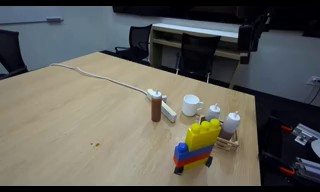
\includegraphics[width=3.8cm]{media/hallucination/lego0.jpg}};
\node[frame] (f2) at (5.9,1.5)  {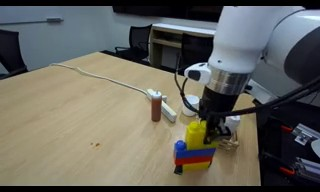
\includegraphics[width=3.8cm]{media/hallucination/lego3.jpg}};
\node[frame] (f3) at (11.8,1.5) {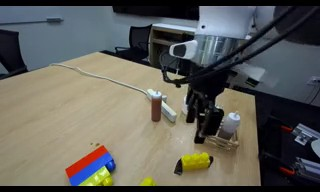
\includegraphics[width=3.8cm]{media/hallucination/lego7.jpg}};
\node[ell] at (2.95,1.5) {$\cdots$};
\node[ell] at (8.85,1.5) {$\cdots$};
% descriptions (real, condensed) -- VLM output, fabrications in red
\node[outtag, text=teal!45!black, anchor=west] at (-2.5,-0.95) {VLM output};
\node[desc] (d1) at (0,-2.0)
  {\textbf{Objects:} yellow, blue and red blocks, and \textcolor{red!75!black}{\bfseries a white and a brown block}. \textbf{Gripper:} not visible. \textbf{Progress:} 1 of 4 stacked, 3 remain.};
\node[desc] (d2) at (5.9,-2.0)
  {\textbf{Objects:} the blocks, stacked. \textbf{Gripper:} holding \textcolor{red!75!black}{\bfseries a white block}. \textbf{Progress:} the block is being placed for stacking.};
\node[desc] (d3) at (11.8,-2.0)
  {\textbf{Objects:} the blocks, scattered again. \textbf{Gripper:} holding \textcolor{red!75!black}{\bfseries a black block}. \textbf{Progress:} the attempt fails; the tower is not taken apart.};
% grade cells -- LLM output
\node[outtag, text=orange!55!black, anchor=west] at (-2.5,-4.35) {LLM output};
\node[grade] (L1) at (0,-5.05)    {{\scriptsize score}\\[1pt]{\large\textbf{1}}};
\node[grade] (L2) at (5.9,-5.05)  {{\scriptsize score}\\[1pt]{\large\textbf{4}}};
\node[grade] (L3) at (11.8,-5.05) {{\scriptsize score}\\[1pt]{\large\textbf{4}}};
% arrows
\draw[->,teal!60!black,thick] (f1) -- (d1);
\draw[->,teal!60!black,thick] (f2) -- (d2);
\draw[->,teal!60!black,thick] (f3) -- (d3);
\draw[->,thick] (d1) -- (L1);
\draw[->,thick] (d2) -- (L2);
\draw[->,thick] (d3) -- (L3);
\draw[->,orange!80!black,thick] (L1) -- node[above=1pt,font=\scriptsize,text=orange!55!black]{$+$ earlier descriptions} (L2);
\draw[->,orange!80!black,thick] (L2) -- node[above=1pt,font=\scriptsize,text=orange!55!black]{$+$ earlier descriptions} (L3);
% stage bands + outer container
\begin{scope}[on background layer]
  \node[fill=teal!5,   rounded corners=4pt, fit=(st1)(tl1)(tl3)(f1)(f3)(d1)(d3), inner sep=8pt] (b1){};
  \node[fill=orange!5, rounded corners=4pt, fit=(st2)(L1)(L3),         inner sep=8pt] (b2){};
  \node[draw=gray!45, line width=0.8pt, rounded corners=6pt, fit=(hdr)(b1)(b2), inner sep=6pt] {};
\end{scope}
\end{tikzpicture}%
}
\caption[A hallucination surviving the pipeline]{A hallucination that survives the two-stage pipeline of Section~\ref{sec:method-real-failures}, shown in the format of Figure~\ref{fig:vlm-llm-pipeline}, on a DROID clip whose task is to unstack a lego tower. The real blocks are yellow, blue and red with a second yellow block on top. The white and brown objects behind them are a cup and a bottle. The VLM's fabrications, in red, report objects that are not there (a white and a brown block), then misread the grasped yellow block as white, and at the end see a black block in an empty gripper. Because each description is stated with confidence, and the reported blocks on the gripper keep changing, the grader is pulled to a full score of four from the fourth frame on, whereas the true progress is closer to two. The arm lifts the top block but then scatters the tower instead of unstacking it. Frames, descriptions, and scores are real outputs.}
\label{fig:vlm-hallucination}
\end{figure}

\chapter{The Loss Study in Detail}
\label{apx:lambda}

The loss study of Section~\ref{sec:results-lora} compares its variants by a single number, the best-checkpoint rank accuracy averaged over the four evaluation splits. This appendix opens that number up. Table~\ref{tab:lora-breakdown} reports every variant of the study at its best checkpoint, with the per-split composition of the demonstration-conditioned aggregate and the demonstration-free aggregate beside it.

\begin{table}[h]
\centering\footnotesize
\caption[The loss study per split]{Every variant of the loss study of Section~\ref{sec:results-lora} at its best checkpoint by the four-split aggregate. The first four columns give the per-split rank accuracy with an in-context demonstration, the last two the aggregates with and without one. The best value per column is in bold.}
\label{tab:lora-breakdown}
\begin{tabular}{@{}lcccccc@{}}
\toprule
 & \multicolumn{4}{c}{with demonstration} & \multicolumn{2}{c}{aggregate} \\
\cmidrule(lr){2-5}\cmidrule(lr){6-7}
Variant & DROID & Robometer & MetaWorld & FailSafe & with & without \\
\midrule
Reweighted $\lambda=0.3$ & 0.572 & \textbf{0.779} & 0.852 & 0.900 & \textbf{0.776} & \textbf{0.757} \\
Reweighted $\lambda=0.5$ & 0.590 & 0.768 & 0.826 & 0.909 & 0.773 & 0.746 \\
CORN $c=0$ & 0.547 & 0.758 & 0.841 & 0.924 & 0.768 & 0.744 \\
CORN $c=0.5$ & 0.544 & 0.713 & 0.811 & 0.932 & 0.750 & 0.732 \\
CORN $c=1.5$ & 0.512 & 0.697 & \textbf{0.882} & 0.918 & 0.752 & 0.747 \\
$\lambda=0.3$ + task dropout & 0.551 & 0.717 & 0.830 & 0.899 & 0.749 & 0.748 \\
$\lambda=0.3$ + KL anchor $0.1$ & \textbf{0.592} & 0.696 & 0.868 & \textbf{0.938} & 0.773 & 0.753 \\
$\lambda=0.3$ + KL anchor $0.3$ & 0.544 & 0.770 & 0.819 & 0.923 & 0.764 & 0.749 \\
\bottomrule
\end{tabular}
\end{table}

Three things stand out in this table. First, the per-split winners scatter, KL $0.1$ takes DROID and FailSafe, the strongest CORN asymmetry takes MetaWorld, yet no variant beats the plain reweighted loss on the aggregate in either mode. Second, DROID is the weakest split for every single variant, roughly $0.51$ to $0.59$ against $0.70$ to $0.94$ everywhere else, the first sign of the pattern the main results confirm at full scale. It also shows what pretraining on ideal demonstrations leaves behind. Robometer never met a real-world failure as a direct training target, so the ability to tell a DROID failure from a success has to be built almost from scratch, and a light adapter on an $18$k sample barely lifts it above chance. It takes the full fine-tunes of Chapter~\ref{sec:results} to raise DROID ranking to $0.734$ (Section~\ref{sec:results-frames}). Third, every best checkpoint falls between steps $500$ and $4{,}000$ of the $7{,}500$-step budget, so the adapters saturate early on this $18$k sample, and the three runs that stopped near step three thousand, CORN $c=0$, $\lambda=0.5$, and the stronger KL anchor, all stopped inside the window where the others peak.

The two aggregate columns carry one more observation. The demonstration lifts every variant of the study, by one to three points, with a single exception: the task-dropout variant, where the two modes land within a tenth of a point of each other. That is the variant that deliberately corrupts the task description on demonstration-carrying samples, so the one configuration built to disturb the language channel of in-context learning is also the one whose demonstration gain disappears. The demonstrations were already paying off at LoRA scale, before any full fine-tune, and the dropout that was meant to strengthen them erased their advantage instead.

\section{Choosing the asymmetry strength}

The main text reports the reweighted loss at a single asymmetry strength, $\lambda = 0.3$, selected against a milder $\lambda = 0.5$ that corrects under-predictions at half strength instead of a third. Table~\ref{tab:lambda-sweep} gives that comparison in full, both variants at their best checkpoint, with and without an in-context demonstration.

\begin{table}[h]
\centering\footnotesize
\caption[Choosing the asymmetry strength]{Rank accuracy of the reweighted loss at two asymmetry strengths, each at its best checkpoint by the four-split aggregate, evaluated with and without an in-context demonstration. The stronger $\lambda = 0.3$ takes the aggregate in both modes, with the differences concentrated on MetaWorld.}
\label{tab:lambda-sweep}
\begin{tabular}{@{}lcccc@{}}
\toprule
 & \multicolumn{2}{c}{with demonstration} & \multicolumn{2}{c}{without} \\
\cmidrule(lr){2-3}\cmidrule(lr){4-5}
Split & $\lambda=0.3$ & $\lambda=0.5$ & $\lambda=0.3$ & $\lambda=0.5$ \\
\midrule
DROID & 0.572 & \textbf{0.590} & 0.517 & \textbf{0.534} \\
Robometer & \textbf{0.779} & 0.768 & 0.794 & \textbf{0.808} \\
MetaWorld & \textbf{0.852} & 0.826 & \textbf{0.791} & 0.717 \\
FailSafe & 0.900 & \textbf{0.909} & \textbf{0.928} & 0.926 \\
\midrule
Aggregate & \textbf{0.776} & 0.773 & \textbf{0.757} & 0.746 \\
\bottomrule
\end{tabular}
\end{table}

The two strengths are close, which is itself the useful finding. Doubling down on the asymmetry costs the reweighted loss essentially nothing in ranking quality, the aggregate favors $\lambda = 0.3$ in both modes, and the one split with a clear gap, MetaWorld without a demonstration, favors it by seven points. This stands in direct contrast to the ordinal family of Table~\ref{tab:lora-breakdown}, whose ranking degrades as its asymmetry $c$ grows, and it is why we keep the stronger setting: at equal or better ranking quality, $\lambda = 0.3$ buys more of the conservatism the loss exists to provide.

\chapter{Length Bias in Video-Based Reward Models}
\label{apx:length-bias}

Section~\ref{sec:method-arch} samples a fixed number of frames from every trajectory instead of passing the raw video to the model. This is what Robometer follows as well, and according to our preliminary tests this is in the right direction. This appendix sheds some light on these decisions. Before adopting Robometer, which came out in March 2026, we were building on RoboReward \citep{roboreward}, which scores a whole video at once instead of feeding separate frames. There, we found that its score was biased by the video length. A reward that reads length as a stand-in for failure is easy for a policy to fool, which is what pushed us toward a fixed frame budget. The study below is small and predates our main experiments based on Robometer, but we consider this study relevant, as it reveals the significance of using frames as input to vision-language reward models.

The confound begins in the training data. RoboReward manufactures most of its negatives by truncating successful episodes, cutting a completed attempt short so that it no longer reaches the goal. Across the 45{,}072 videos of its released dataset, 11{,}116 of the lower-reward examples are these temporal clips, the same task with the video cut off partway, against only 3{,}228 counterfactual relabels. The average full episode runs about 31 seconds and the average clip about 9.5. Shorter therefore correlates with failure by construction. The effect is amplified at inference, because the video-loading path samples frames at a fixed rate of two per second by default, so a shorter clip is also seen through fewer frames. A model trained this way can pick up a shortcut, that few frames means failure, which has nothing to do with the task itself.

To probe RoboReward-8B for this shortcut, we evaluated the model as a binary classifier, asking a simple yes-or-no question for each clip: did the attempt succeed? We framed the evaluation this way for two reasons. First, the clips in our dataset carry a binary ground truth, they are either genuine successes or truncated failures, so metrics like recall and the confusion matrix require a binary prediction to be meaningful. Second, this mirrors how such a reward is actually used in practice; a policy ultimately acts on a hard success decision dictated by a threshold, not a soft continuous score. 

While we inherited the one-to-five scoring concept from RoboReward, we adapted it to fit our approach. This introduced two key differences:
\begin{itemize}
    \item \textbf{Granularity:} RoboReward assigns a single holistic score to the entire trajectory, where 5 is a clean success and 1 is no progress at all. In contrast, our model outputs a dense, per-frame progress signal. 
    \item \textbf{Specificity:} RoboReward relies on more abstract definitions for its intermediate scores (2, 3, and 4). We explicitly defined these intermediate states later in our own implementation. 
\end{itemize}

To convert RoboReward's trajectory-level score into a binary verdict for our confusion matrices, we imposed a threshold of 3.5. Any prediction of 3.5 or higher is counted as a success, while anything below is a failure. We chose this deliberately lenient cutoff for this specific analysis so that a ``mostly successful'' score of 4 still passes as a success. Later, in our configuration, we enforced a stricter approach by accepting only a 5 as a success. It should be noted, however, that the length effect we report holds true regardless of where this initial threshold is drawn.

\begin{figure}[h]
\centering
\begin{minipage}[b]{0.49\textwidth}
  \centering
  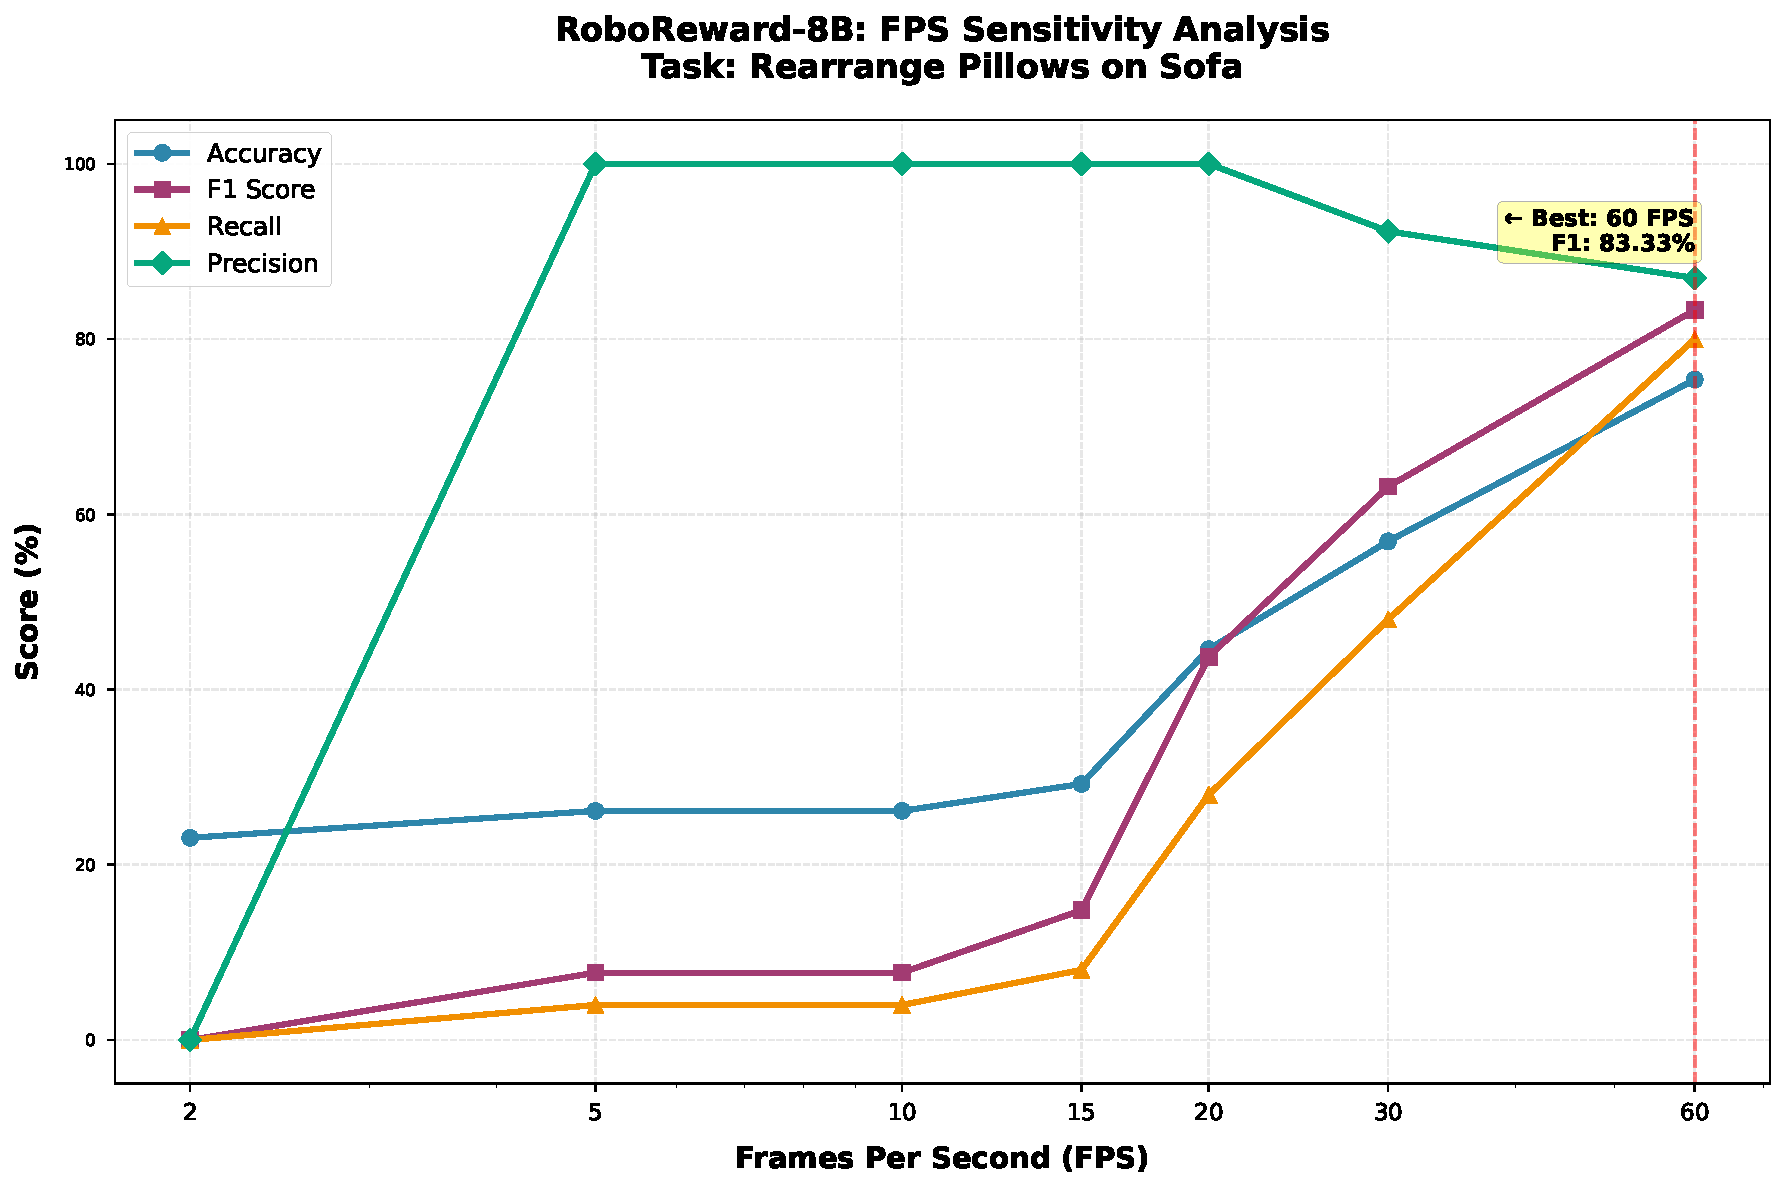
\includegraphics[width=\textwidth]{media/length-bias/fps_sweep.pdf}\\
  {\footnotesize (a) Frame-sampling sweep}
\end{minipage}\hfill
\begin{minipage}[b]{0.49\textwidth}
  \centering
  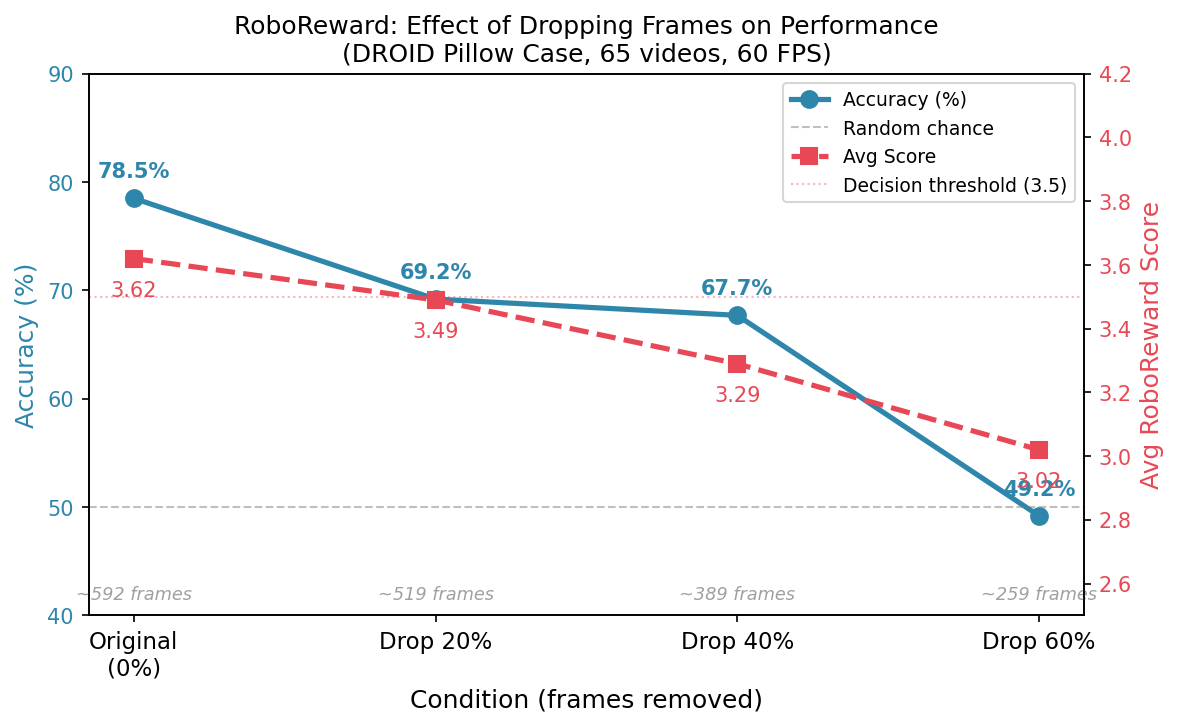
\includegraphics[width=\textwidth]{media/length-bias/frame_drop.png}\\
  {\footnotesize (b) Frame drop at fixed rate}
\end{minipage}
\caption[RoboReward scores video length, not content]{RoboReward-8B scores video length as much as content, on 65 DROID pillow-rearranging clips (50 success, 15 failure). \emph{(a)} As the frame-sampling rate falls, recall collapses toward zero, so successful attempts read as failures purely because they are seen through fewer frames. \emph{(b)} Holding the rate fixed at 60 frames per second and instead dropping a uniform fraction of the frames, with the visible content unchanged, accuracy falls from 78.5 to 49.2 percent and the mean score crosses the 3.5 success cutoff (scores at or above 3.5 count as a predicted success), flipping 25 of the 65 predictions. This is the length shortcut that motivates giving RoboRef a fixed frame budget in Section~\ref{sec:method-arch}.}
\label{fig:length-bias}
\end{figure}

First we swept the frame-sampling rate. On a set of 65 DROID clips of a pillow-rearranging task, 50 successes and 15 failures recorded at 60 frames per second, we varied the sampling rate from the library default up to the native rate and read off the verdict at each rate. At the default of two frames per second the model called every one of the 50 successful clips a failure, a recall of zero, and only as the frame count climbed did success become recognizable, reaching a recall of 80 percent near the native rate. Figure~\ref{fig:length-bias}~(a) shows the sweep. We saw the same collapse on data drawn from RoboReward's own training distribution, where recall moved from 5 percent at two frames per second to 80 percent at the native ten. The rate that worked best tracked each dataset's native frame count and not any fixed value, which is what a frame-count artifact would predict and genuine task understanding would not.

The sweep changes two things at once, the number of frames and the timestamps the model reads, so we ran a cleaner test that varies only the frame count. Holding the sampling rate fixed at 60 frames per second, we extracted every frame and then dropped a uniform fraction of them before scoring, leaving the visible content otherwise untouched. Figure~\ref{fig:length-bias}~(b) shows what happens. Removing frames drives accuracy down from 78.5 percent on the full clips to 49.2 percent, no better than chance. The mean score falls with it, from 3.62 on the full clips, comfortably on the success side of the 3.5 cutoff, down to 3.02, now on the failure side, so the average clip flips its verdict from success to failure. A quarter of the individual predictions, 25 of the 65, flip the same way, with no change at all to what the video shows. The same attempt, seen through fewer frames, reads as a failure.

We present these results with two important notes. The samples are small and imbalanced, 65 clips with only 15 failures, so these are pilot-scale numbers on a single prior model, not a controlled benchmark. Also, the study probes RoboReward, not our own model, so it only motivates a design decision. That decision is to hand the reward model a fixed number of frames per trajectory, eight in Robometer and sixteen in ours, evenly spaced regardless of how long the attempt lasts. A shorter or longer episode is then always seen through the same window, so length can no longer stand in for progress, and the model is forced to judge the attempt on what the frames show.

\chapter{The Conditional-Mean Readout of the Progress Head}
\label{apx:condmean}

The progress columns of the out-of-distribution evaluation, Table~\ref{tab:offline-ood}, are decoded differently from every other number in this thesis, and this appendix explains why, shows the model outputs behind the choice, and answers the objection the choice raises. Robometer's progress head is discrete. It places a probability on each of ten progress bins, and the released pipeline turns this into a scalar by taking the expectation, the probability-weighted mean of the bin centers. The in-distribution results of Tables~\ref{tab:offline-id-rank} and~\ref{tab:offline-id-succ} use that same readout. On the held-out-robot set it stops being usable for the fine-tuned models, because their bin distributions turn bimodal, with a large share of the mass parked on the lowest bin and most of the remainder concentrated near the top. The expectation of such a mixture lands between the two modes, at a value the model itself considers unlikely, and more importantly it multiplies the informative part of the prediction by one minus the lowest-bin mass. Whether the ordering of clips survives that multiplication depends entirely on how that mass behaves across clips. Figure~\ref{fig:bimodal-bins} shows the shape directly for RoboRef-Asym, averaged over thirty successful and thirty failed clips of a manipulation task from its training corpus.

\begin{figure*}[h]
  \centering
  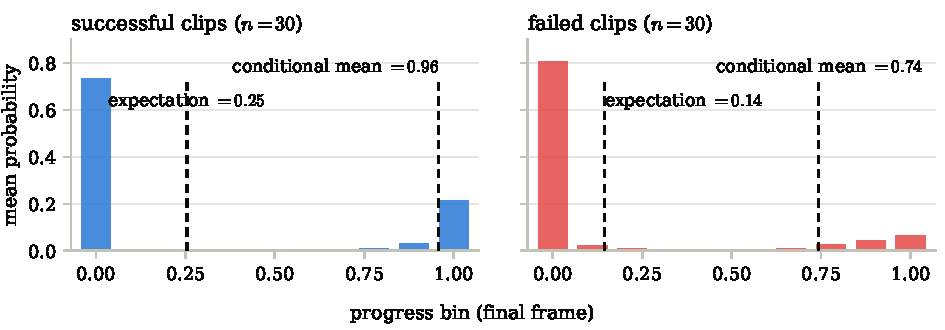
\includegraphics[width=0.93\textwidth]{media/results/bimodal_bins_readouts.pdf}
  \caption[Bimodal progress-bin distributions]{The average final-frame bin distribution of the asymmetric fine-tune on clips of a training task, split by outcome. Both distributions are bimodal, with a large share of the probability on the lowest bin and most of the rest near the top. The expectation lands between the two modes, at a value the model itself gives almost no probability, and reads a genuine success at $0.25$. The conditional mean ignores the lowest bin and reads the same clips at $0.96$ and $0.74$, the right order with a wider gap between the outcomes.}
  \label{fig:bimodal-bins}
\end{figure*}

We therefore decode the progress head with the conditional mean, the same expectation taken after the lowest bin is dropped and the remaining nine renormalized. It answers a narrower question, namely how far the clip has progressed given that the model sees progress at all. Table~\ref{tab:offline-ood} applies it to every model. For the baseline this changes nothing, its distributions are unimodal with almost no mass on the lowest bin, and its two progress columns move by less than a point under the new decode, so the transform cannot be favoring our models by construction. For the fine-tuned models the effect is large. The asymmetric model's Kendall's $\tau$ on this set is $0.16$ under the plain expectation and the $0.58$ reported in the table under the conditional mean.

The natural objection is that the in-distribution results of Tables~\ref{tab:offline-id-rank} and~\ref{tab:offline-id-succ}, which keep the plain expectation, should suffer from the same problem, since the same failure-heavy training produced the same bimodal heads there. They do not, and the reason is that rank metrics are indifferent to any distortion that preserves order. In distribution the lowest-bin mass is systematic, failures carry visibly more of it than successes, so scaling every score by one minus that mass compresses the numbers but keeps them in the right order, and rank accuracy and $\tau$ cannot tell the difference. On held-out robots the same mass stops tracking the task and starts tracking the unfamiliar embodiment. Measured on the held-out-robot set for the asymmetric fine-tune, successful clips carry a mean lowest-bin mass of $0.70$ and failed ones $0.71$, a gap of $0.01$ between the classes against a within-class spread of $0.07$. A factor seven times as noisy as it is informative scrambles any ordering it multiplies, which is what the plain expectation shows, and dividing it out is what restores it. Figure~\ref{fig:hedge-mass} shows the contrast directly. The same effect sits behind part~(a) of Figure~\ref{fig:offline-qual}, where the completed out-of-distribution success is read at $0.21$ by the plain expectation.

\begin{figure*}[h]
  \centering
  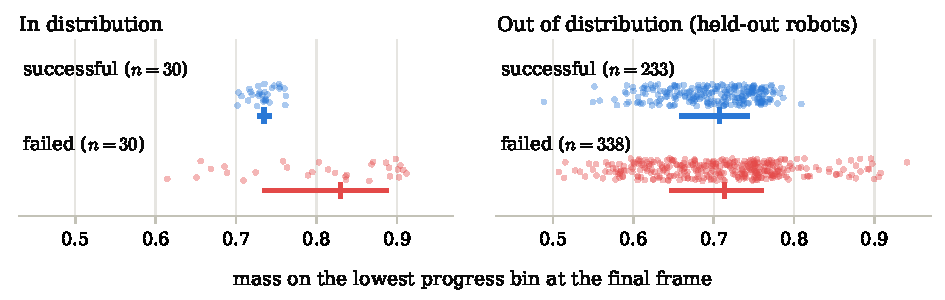
\includegraphics[width=0.93\textwidth]{media/results/hedge_mass_id_vs_ood.pdf}
  \caption[Why the conditional mean is needed only out of distribution]{Why the conditional mean is needed out of distribution and not in distribution, shown on the asymmetric fine-tune. Each dot is one clip. Its position shows how much probability the model puts on the lowest progress bin at the final frame, in other words how strongly the model votes that the clip shows no progress. The plain expectation scales a clip's score by one minus this value, so clips further to the right end up with smaller scores. The short vertical line under each group marks the median clip and the horizontal bar spans the middle half of the group. In distribution (left, clips of a training task) the vote is accurate. Failed clips sit clearly to the right of successful ones, their scores shrink more, and the final scores still rank successes above failures. On the held-out robots of Table~\ref{tab:offline-ood} (right) successful and failed clips receive almost the same vote on average while individual clips of either kind vary widely, so the shrinking is essentially random and it shuffles the final scores. The conditional mean removes this factor, which is what restores the ranking.}
  \label{fig:hedge-mass}
\end{figure*}

\chapter{Reward Received During MetaWorld Training}
\label{apx:mw-reward}

This appendix expands the reward-hacking analysis that Section~\ref{sec:results-rl-mw} summarizes. Figure~\ref{fig:mw-reward} plots the reward the policy actually received during training, the mean per-step value the reward model returned, for our three RoboRef fine-tunes and the released Robometer-4B, which all read the same success head and so pay on one comparable scale. This is the model's own reward and not the true task reward, and the success rates of Figure~\ref{fig:mw-rl} remain the ground truth throughout.

On Coffee-Push the released Robometer-4B pays the policy the most reward of any model, by a wide margin, roughly $0.04$ per step against the asymmetric fine-tunes' $0.01$ to $0.02$, while training a policy whose true success rate is zero. A reward that grows while success does not is the signature of reward hacking, since the policy has found the false positives the model's offline overconfidence promised (Figure~\ref{fig:offline-qual}) and learned to manufacture them, collecting a reward it never earned. The asymmetric fine-tunes tell the opposite story, paying a smaller reward that climbs together with true success, the shape of a signal being earned, not gamed, while RoboRef-Std fires rarely and pays almost nothing, moving the policy little. The difference between Robometer-4B and RoboRef-Std is our failure data, which taught the latter to reject the near-misses MetaWorld policies actually produce, so the blatant false positives the released model farms are gone. What remains is the opposite problem, a reward so hesitant that it underpays genuine progress, and this starves the policy where the released model misleads it. The dense-reward baselines sit on scales that cannot be read against these. In short, the reward a policy collects is a poor proxy for the policy it becomes, and holding the two apart is precisely the job of the conservative loss.


\begin{figure*}[h]
\centering
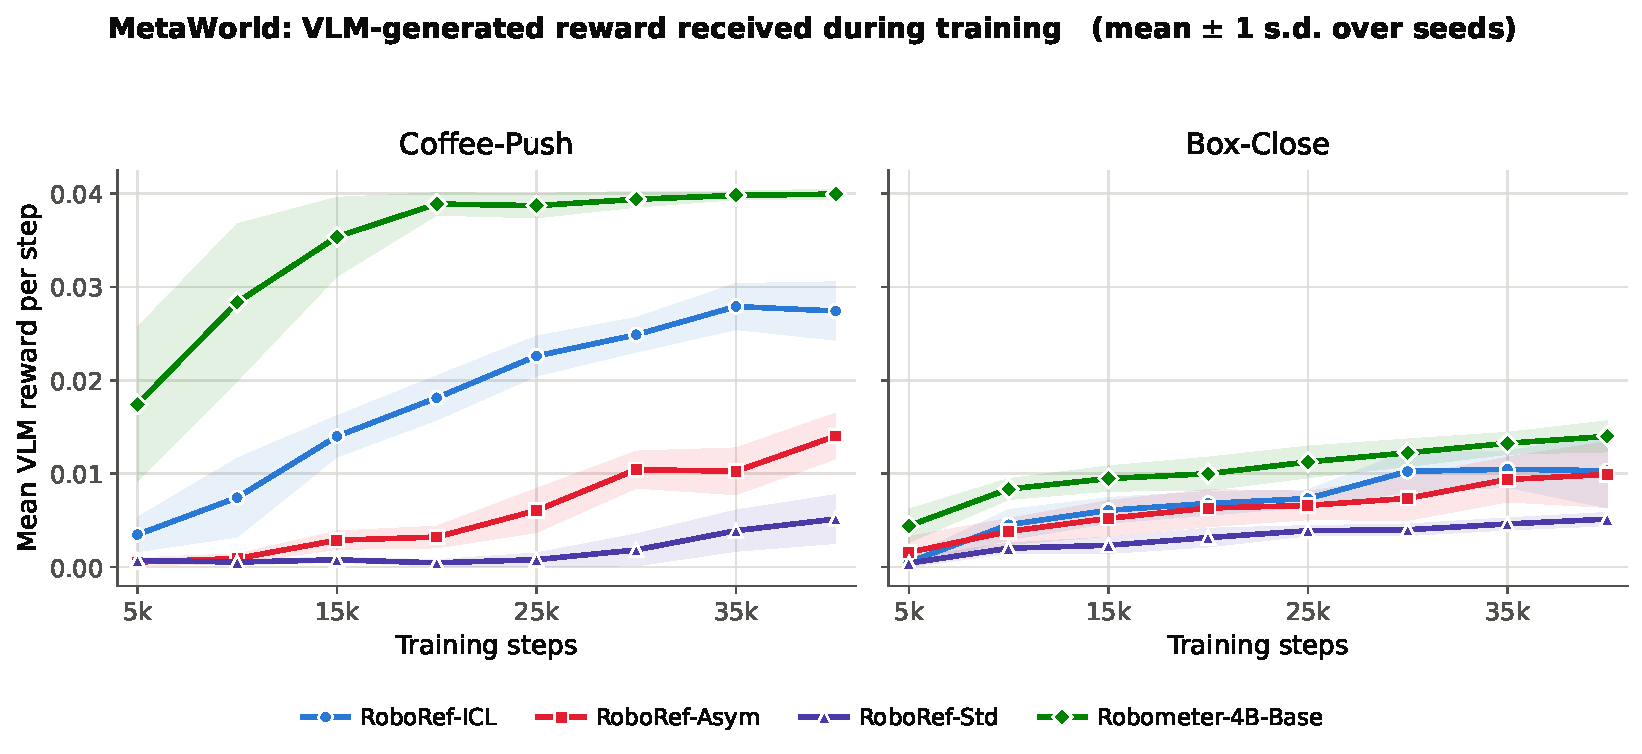
\includegraphics[width=\textwidth]{media/results/metaworld_reward.pdf}
\caption[VLM reward received during MetaWorld training]{The vision-language reward the policy received during training, mean per-step value returned by the reward model, for our three RoboRef fine-tunes and the released Robometer-4B, which share one success-probability scale and are therefore comparable. This is the model's own reward, not the true task reward of Figure~\ref{fig:mw-rl}. On Coffee-Push the released Robometer-4B pays the most reward of any model yet its policy never succeeds, the mark of farmed false positives; the asymmetric fine-tunes pay a smaller reward that rises with genuine success.}
\label{fig:mw-reward}
\end{figure*}

Lastly, we underline that the result is not an artifact of how the comparison is implemented. Every reward in the figure is calibrated by the same procedure and held to the same minimum length, and every baseline still fails, so the advantage can only sit in the reward itself, its refusal to pay out on the near-misses a policy will otherwise learn to manufacture.


\chapter{Examples of Generated Failure Data}
\label{apx:gallery}

This appendix shows a sample of the failure trajectories we generate in simulation, the data described in Section~\ref{sec:method-sim-failures}. Each example is a short filmstrip of a single failed attempt, and the number above each frame is its ground-truth progress score, read directly from the simulator state. The scores run from $1$ (no progress) to $5$ (success), so a failed attempt never exceeds $4$.

We group the examples by the score the attempt reaches, so each block illustrates what a given level of partial progress looks like across different tasks and different ways of failing. The failure modes the generator can use depend on how far the attempt gets. Early failures look like random flailing or motion in the wrong direction, mid-progress failures hold an object and then freeze or push it the wrong way, and near-complete failures grasp or place the object and then drop or misplace it at the last moment. The scores follow the behavior, including downward when an object is dropped, which is the property a monotone $t/T$ label cannot capture.

\section{Tasks and failure modes}

Both simulated benchmarks generate failures by injecting a fault into a scripted policy, as described in Section~\ref{sec:method-sim-failures}. The kind of failure that comes out depends on the task family and the target score. Table~\ref{tab:sim-modes} lists the nine noise modes we use in MetaWorld \citep{yu_meta-world_2019} and where each applies, and Table~\ref{tab:sim-tasks} lists the tasks by family.

\begin{table}[t]
\centering\footnotesize
\caption[MetaWorld noise modes]{The nine MetaWorld noise modes and the family and score at which each is applied. Scores~1 and~2 use the same modes across every family; the higher scores are family-specific.}
\label{tab:sim-modes}
\begin{tabular}{@{}p{2.4cm}p{5.9cm}p{4.7cm}@{}}
\toprule
Mode & Behavior & Applied at \\
\midrule
random & fully random actions & score 1 (all families) \\
wrong-direction & a strong bias away from the goal & score 1 (all); score 3 (grasp-and-move) \\
freeze & the arm holds its position & scores 2--4 (all families) \\
drop & the gripper is forced open mid-transport & score 3 (grasp-and-move) \\
late-drop & the gripper is forced open near the goal & score 4 (grasp-and-move) \\
misplace & the expert action with a small offset near the goal & score 4 (grasp-and-move, push-and-sweep) \\
lift-away & the arm lifts off and loses contact & score 3 (push-and-sweep) \\
push-sideways & the arm pushes perpendicular to the goal & scores 3--4 (push-and-sweep) \\
partial-actuation & the expert drives the mechanism most of the way, then stalls & score 4 (mechanism, press) \\
\bottomrule
\end{tabular}
\end{table}

\begin{table}[t]
\centering\footnotesize
\caption[MetaWorld tasks by family]{The 46 MetaWorld tasks by family, with the scores each family covers. Mechanism and press tasks skip score~3, whose single actuation has no meaningful partial state.}
\label{tab:sim-tasks}
\begin{tabular}{@{}p{2.3cm}cp{9.0cm}@{}}
\toprule
Family & Scores & Tasks \\
\midrule
Grasp-and-move & 1--4 & assembly, basketball, bin-picking, box-close, coffee-pull, hammer, hand-insert, pick-out-of-hole, pick-place, pick-place-wall, shelf-place, stick-pull, stick-push \\
\addlinespace
Push-and-sweep & 1--4 & coffee-push, plate-slide, plate-slide-side, plate-slide-back, plate-slide-back-side, push, push-wall, push-back, soccer, sweep, sweep-into \\
\addlinespace
Mechanism & 1, 2, 4 & dial-turn, disassemble, door-open, door-close, door-lock, door-unlock, drawer-open, drawer-close, faucet-open, faucet-close, handle-press, handle-press-side, handle-pull, handle-pull-side, lever-pull, window-open, window-close \\
\addlinespace
Press & 1, 2, 4 & button-press, button-press-wall, button-press-topdown, button-press-topdown-wall, coffee-button \\
\bottomrule
\end{tabular}
\end{table}

FailSafe \citep{lin_failsafe_2025} adds three ManiSkill \citep{tao_maniskill3_2024} tasks, \texttt{FailPickCube} (lift a cube to a goal), \texttt{FailPushCube} (push a cube to a goal), and \texttt{FailStackCube} (stack a red cube on a green one), scored on the same one-to-five scale. Each task is driven by a scripted multi-stage planner, reach, grasp, lift, align, place, and a fault is injected at a chosen stage. The stage sets the score, so a fault early in the plan yields a low score and one at the last stage a near-complete score-4 failure. The injected fault fits the stage, a grasp that is then released or frozen, a push that stalls or veers off, or a cube carried and dropped just short of the target. Stacking is the only FailSafe task with a meaningful score~3, a cube grasped and held or carried but not yet placed.

\section{Score 1: no meaningful progress}
{\centering
\setlength{\tabcolsep}{1pt}\renewcommand{\arraystretch}{0.5}
\begin{tabular}{@{}cccccccc@{}}
{\scriptsize 1} & {\scriptsize 1} & {\scriptsize 1} & {\scriptsize 1} & {\scriptsize 1} & {\scriptsize 1} & {\scriptsize 1} & {\scriptsize 1} \\

\includegraphics[width=0.118\textwidth]{media/appendix/s1_window/f0.jpg} &

\includegraphics[width=0.118\textwidth]{media/appendix/s1_window/f1.jpg} &

\includegraphics[width=0.118\textwidth]{media/appendix/s1_window/f2.jpg} &

\includegraphics[width=0.118\textwidth]{media/appendix/s1_window/f3.jpg} &

\includegraphics[width=0.118\textwidth]{media/appendix/s1_window/f4.jpg} &

\includegraphics[width=0.118\textwidth]{media/appendix/s1_window/f5.jpg} &

\includegraphics[width=0.118\textwidth]{media/appendix/s1_window/f6.jpg} &

\includegraphics[width=0.118\textwidth]{media/appendix/s1_window/f7.jpg} \\
\end{tabular}\\[2pt]
{\footnotesize Window-close, random actions.}\par}
\vspace{8pt}
{\centering
\setlength{\tabcolsep}{1pt}\renewcommand{\arraystretch}{0.5}
\begin{tabular}{@{}cccccccc@{}}
{\scriptsize 1} & {\scriptsize 1} & {\scriptsize 1} & {\scriptsize 1} & {\scriptsize 1} & {\scriptsize 1} & {\scriptsize 1} & {\scriptsize 1} \\

\includegraphics[width=0.118\textwidth]{media/appendix/s1_door/f0.jpg} &

\includegraphics[width=0.118\textwidth]{media/appendix/s1_door/f1.jpg} &

\includegraphics[width=0.118\textwidth]{media/appendix/s1_door/f2.jpg} &

\includegraphics[width=0.118\textwidth]{media/appendix/s1_door/f3.jpg} &

\includegraphics[width=0.118\textwidth]{media/appendix/s1_door/f4.jpg} &

\includegraphics[width=0.118\textwidth]{media/appendix/s1_door/f5.jpg} &

\includegraphics[width=0.118\textwidth]{media/appendix/s1_door/f6.jpg} &

\includegraphics[width=0.118\textwidth]{media/appendix/s1_door/f7.jpg} \\
\end{tabular}\\[2pt]
{\footnotesize Door-open, wanders off, never reaches the door.}\par}
\vspace{8pt}
{\centering
\setlength{\tabcolsep}{1pt}\renewcommand{\arraystretch}{0.5}
\begin{tabular}{@{}cccccccc@{}}
{\scriptsize 1} & {\scriptsize 1} & {\scriptsize 1} & {\scriptsize 1} & {\scriptsize 1} & {\scriptsize 1} & {\scriptsize 1} & {\scriptsize 1} \\

\includegraphics[width=0.118\textwidth]{media/appendix/s1_push/f0.jpg} &

\includegraphics[width=0.118\textwidth]{media/appendix/s1_push/f1.jpg} &

\includegraphics[width=0.118\textwidth]{media/appendix/s1_push/f2.jpg} &

\includegraphics[width=0.118\textwidth]{media/appendix/s1_push/f3.jpg} &

\includegraphics[width=0.118\textwidth]{media/appendix/s1_push/f4.jpg} &

\includegraphics[width=0.118\textwidth]{media/appendix/s1_push/f5.jpg} &

\includegraphics[width=0.118\textwidth]{media/appendix/s1_push/f6.jpg} &

\includegraphics[width=0.118\textwidth]{media/appendix/s1_push/f7.jpg} \\
\end{tabular}\\[2pt]
{\footnotesize Push, moves the wrong way.}\par}
\vspace{8pt}
{\centering
\setlength{\tabcolsep}{1pt}\renewcommand{\arraystretch}{0.5}
\begin{tabular}{@{}cccccccc@{}}
{\scriptsize 1} & {\scriptsize 1} & {\scriptsize 1} & {\scriptsize 1} & {\scriptsize 1} & {\scriptsize 1} & {\scriptsize 1} & {\scriptsize 1} \\

\includegraphics[width=0.118\textwidth]{media/appendix/s1_hammer/f0.jpg} &

\includegraphics[width=0.118\textwidth]{media/appendix/s1_hammer/f1.jpg} &

\includegraphics[width=0.118\textwidth]{media/appendix/s1_hammer/f2.jpg} &

\includegraphics[width=0.118\textwidth]{media/appendix/s1_hammer/f3.jpg} &

\includegraphics[width=0.118\textwidth]{media/appendix/s1_hammer/f4.jpg} &

\includegraphics[width=0.118\textwidth]{media/appendix/s1_hammer/f5.jpg} &

\includegraphics[width=0.118\textwidth]{media/appendix/s1_hammer/f6.jpg} &

\includegraphics[width=0.118\textwidth]{media/appendix/s1_hammer/f7.jpg} \\
\end{tabular}\\[2pt]
{\footnotesize Hammer, random actions.}\par}
\vspace{8pt}

\bigskip

\section{Score 2: object approached but not engaged}
{\centering
\setlength{\tabcolsep}{1pt}\renewcommand{\arraystretch}{0.5}
\begin{tabular}{@{}cccccccc@{}}
{\scriptsize 2} & {\scriptsize 2} & {\scriptsize 2} & {\scriptsize 2} & {\scriptsize 2} & {\scriptsize 2} & {\scriptsize 2} & {\scriptsize 2} \\

\includegraphics[width=0.118\textwidth]{media/appendix/s2_faucet/f0.jpg} &

\includegraphics[width=0.118\textwidth]{media/appendix/s2_faucet/f1.jpg} &

\includegraphics[width=0.118\textwidth]{media/appendix/s2_faucet/f2.jpg} &

\includegraphics[width=0.118\textwidth]{media/appendix/s2_faucet/f3.jpg} &

\includegraphics[width=0.118\textwidth]{media/appendix/s2_faucet/f4.jpg} &

\includegraphics[width=0.118\textwidth]{media/appendix/s2_faucet/f5.jpg} &

\includegraphics[width=0.118\textwidth]{media/appendix/s2_faucet/f6.jpg} &

\includegraphics[width=0.118\textwidth]{media/appendix/s2_faucet/f7.jpg} \\
\end{tabular}\\[2pt]
{\footnotesize Faucet-open, reaches then freezes.}\par}
\vspace{8pt}
{\centering
\setlength{\tabcolsep}{1pt}\renewcommand{\arraystretch}{0.5}
\begin{tabular}{@{}cccccccc@{}}
{\scriptsize 1} & {\scriptsize 1} & {\scriptsize 1} & {\scriptsize 1} & {\scriptsize 2} & {\scriptsize 2} & {\scriptsize 2} & {\scriptsize 2} \\

\includegraphics[width=0.118\textwidth]{media/appendix/s2_door/f0.jpg} &

\includegraphics[width=0.118\textwidth]{media/appendix/s2_door/f1.jpg} &

\includegraphics[width=0.118\textwidth]{media/appendix/s2_door/f2.jpg} &

\includegraphics[width=0.118\textwidth]{media/appendix/s2_door/f3.jpg} &

\includegraphics[width=0.118\textwidth]{media/appendix/s2_door/f4.jpg} &

\includegraphics[width=0.118\textwidth]{media/appendix/s2_door/f5.jpg} &

\includegraphics[width=0.118\textwidth]{media/appendix/s2_door/f6.jpg} &

\includegraphics[width=0.118\textwidth]{media/appendix/s2_door/f7.jpg} \\
\end{tabular}\\[2pt]
{\footnotesize Door-open, reaches then freezes.}\par}
\vspace{8pt}
{\centering
\setlength{\tabcolsep}{1pt}\renewcommand{\arraystretch}{0.5}
\begin{tabular}{@{}cccccccc@{}}
{\scriptsize 1} & {\scriptsize 1} & {\scriptsize 1} & {\scriptsize 2} & {\scriptsize 2} & {\scriptsize 2} & {\scriptsize 2} & {\scriptsize 2} \\

\includegraphics[width=0.118\textwidth]{media/appendix/s2_sweep/f0.jpg} &

\includegraphics[width=0.118\textwidth]{media/appendix/s2_sweep/f1.jpg} &

\includegraphics[width=0.118\textwidth]{media/appendix/s2_sweep/f2.jpg} &

\includegraphics[width=0.118\textwidth]{media/appendix/s2_sweep/f3.jpg} &

\includegraphics[width=0.118\textwidth]{media/appendix/s2_sweep/f4.jpg} &

\includegraphics[width=0.118\textwidth]{media/appendix/s2_sweep/f5.jpg} &

\includegraphics[width=0.118\textwidth]{media/appendix/s2_sweep/f6.jpg} &

\includegraphics[width=0.118\textwidth]{media/appendix/s2_sweep/f7.jpg} \\
\end{tabular}\\[2pt]
{\footnotesize Sweep-into, touches then freezes.}\par}
\vspace{8pt}
{\centering
\setlength{\tabcolsep}{1pt}\renewcommand{\arraystretch}{0.5}
\begin{tabular}{@{}cccccccc@{}}
{\scriptsize 1} & {\scriptsize 1} & {\scriptsize 1} & {\scriptsize 1} & {\scriptsize 2} & {\scriptsize 2} & {\scriptsize 2} & {\scriptsize 2} \\

\includegraphics[width=0.118\textwidth]{media/appendix/s2_drawer/f0.jpg} &

\includegraphics[width=0.118\textwidth]{media/appendix/s2_drawer/f1.jpg} &

\includegraphics[width=0.118\textwidth]{media/appendix/s2_drawer/f2.jpg} &

\includegraphics[width=0.118\textwidth]{media/appendix/s2_drawer/f3.jpg} &

\includegraphics[width=0.118\textwidth]{media/appendix/s2_drawer/f4.jpg} &

\includegraphics[width=0.118\textwidth]{media/appendix/s2_drawer/f5.jpg} &

\includegraphics[width=0.118\textwidth]{media/appendix/s2_drawer/f6.jpg} &

\includegraphics[width=0.118\textwidth]{media/appendix/s2_drawer/f7.jpg} \\
\end{tabular}\\[2pt]
{\footnotesize Drawer-open, reaches the handle but never grips it.}\par}
\vspace{8pt}

\bigskip

\section{Score 3: object engaged, partial progress}
{\centering
\setlength{\tabcolsep}{1pt}\renewcommand{\arraystretch}{0.5}
\begin{tabular}{@{}cccccccc@{}}
{\scriptsize 1} & {\scriptsize 2} & {\scriptsize 2} & {\scriptsize 2} & {\scriptsize 3} & {\scriptsize 3} & {\scriptsize 3} & {\scriptsize 3} \\

\includegraphics[width=0.118\textwidth]{media/appendix/s3_bball/f0.jpg} &

\includegraphics[width=0.118\textwidth]{media/appendix/s3_bball/f1.jpg} &

\includegraphics[width=0.118\textwidth]{media/appendix/s3_bball/f2.jpg} &

\includegraphics[width=0.118\textwidth]{media/appendix/s3_bball/f3.jpg} &

\includegraphics[width=0.118\textwidth]{media/appendix/s3_bball/f4.jpg} &

\includegraphics[width=0.118\textwidth]{media/appendix/s3_bball/f5.jpg} &

\includegraphics[width=0.118\textwidth]{media/appendix/s3_bball/f6.jpg} &

\includegraphics[width=0.118\textwidth]{media/appendix/s3_bball/f7.jpg} \\
\end{tabular}\\[2pt]
{\footnotesize Basketball, grasps the ball but never lifts it to the hoop.}\par}
\vspace{8pt}
{\centering
\setlength{\tabcolsep}{1pt}\renewcommand{\arraystretch}{0.5}
\begin{tabular}{@{}cccccccc@{}}
{\scriptsize 1} & {\scriptsize 1} & {\scriptsize 1} & {\scriptsize 2} & {\scriptsize 3} & {\scriptsize 3} & {\scriptsize 3} & {\scriptsize 3} \\

\includegraphics[width=0.118\textwidth]{media/appendix/s3_pickpl/f0.jpg} &

\includegraphics[width=0.118\textwidth]{media/appendix/s3_pickpl/f1.jpg} &

\includegraphics[width=0.118\textwidth]{media/appendix/s3_pickpl/f2.jpg} &

\includegraphics[width=0.118\textwidth]{media/appendix/s3_pickpl/f3.jpg} &

\includegraphics[width=0.118\textwidth]{media/appendix/s3_pickpl/f4.jpg} &

\includegraphics[width=0.118\textwidth]{media/appendix/s3_pickpl/f5.jpg} &

\includegraphics[width=0.118\textwidth]{media/appendix/s3_pickpl/f6.jpg} &

\includegraphics[width=0.118\textwidth]{media/appendix/s3_pickpl/f7.jpg} \\
\end{tabular}\\[2pt]
{\footnotesize Pick-place, picks up the puck then drops it.}\par}
\vspace{8pt}
{\centering
\setlength{\tabcolsep}{1pt}\renewcommand{\arraystretch}{0.5}
\begin{tabular}{@{}cccccccc@{}}
{\scriptsize 1} & {\scriptsize 1} & {\scriptsize 1} & {\scriptsize 2} & {\scriptsize 3} & {\scriptsize 3} & {\scriptsize 3} & {\scriptsize 3} \\

\includegraphics[width=0.118\textwidth]{media/appendix/s3_push/f0.jpg} &

\includegraphics[width=0.118\textwidth]{media/appendix/s3_push/f1.jpg} &

\includegraphics[width=0.118\textwidth]{media/appendix/s3_push/f2.jpg} &

\includegraphics[width=0.118\textwidth]{media/appendix/s3_push/f3.jpg} &

\includegraphics[width=0.118\textwidth]{media/appendix/s3_push/f4.jpg} &

\includegraphics[width=0.118\textwidth]{media/appendix/s3_push/f5.jpg} &

\includegraphics[width=0.118\textwidth]{media/appendix/s3_push/f6.jpg} &

\includegraphics[width=0.118\textwidth]{media/appendix/s3_push/f7.jpg} \\
\end{tabular}\\[2pt]
{\footnotesize Push the puck to the goal, then slides it sideways instead.}\par}
\vspace{8pt}
{\centering
\setlength{\tabcolsep}{1pt}\renewcommand{\arraystretch}{0.5}
\begin{tabular}{@{}cccccccc@{}}
{\scriptsize 1} & {\scriptsize 1} & {\scriptsize 1} & {\scriptsize 2} & {\scriptsize 3} & {\scriptsize 3} & {\scriptsize 2} & {\scriptsize 2} \\

\includegraphics[width=0.118\textwidth]{media/appendix/s3_coffee/f0.jpg} &

\includegraphics[width=0.118\textwidth]{media/appendix/s3_coffee/f1.jpg} &

\includegraphics[width=0.118\textwidth]{media/appendix/s3_coffee/f2.jpg} &

\includegraphics[width=0.118\textwidth]{media/appendix/s3_coffee/f3.jpg} &

\includegraphics[width=0.118\textwidth]{media/appendix/s3_coffee/f4.jpg} &

\includegraphics[width=0.118\textwidth]{media/appendix/s3_coffee/f5.jpg} &

\includegraphics[width=0.118\textwidth]{media/appendix/s3_coffee/f6.jpg} &

\includegraphics[width=0.118\textwidth]{media/appendix/s3_coffee/f7.jpg} \\
\end{tabular}\\[2pt]
{\footnotesize Coffee-push, pushes partway then lifts away.}\par}
\vspace{8pt}

\bigskip

\section{Score 4: near-complete but ultimately fails}
{\centering
\setlength{\tabcolsep}{1pt}\renewcommand{\arraystretch}{0.5}
\begin{tabular}{@{}cccccccc@{}}
{\scriptsize 1} & {\scriptsize 1} & {\scriptsize 2} & {\scriptsize 3} & {\scriptsize 4} & {\scriptsize 3} & {\scriptsize 3} & {\scriptsize 3} \\

\includegraphics[width=0.118\textwidth]{media/appendix/s4_pickpl/f0.jpg} &

\includegraphics[width=0.118\textwidth]{media/appendix/s4_pickpl/f1.jpg} &

\includegraphics[width=0.118\textwidth]{media/appendix/s4_pickpl/f2.jpg} &

\includegraphics[width=0.118\textwidth]{media/appendix/s4_pickpl/f3.jpg} &

\includegraphics[width=0.118\textwidth]{media/appendix/s4_pickpl/f4.jpg} &

\includegraphics[width=0.118\textwidth]{media/appendix/s4_pickpl/f5.jpg} &

\includegraphics[width=0.118\textwidth]{media/appendix/s4_pickpl/f6.jpg} &

\includegraphics[width=0.118\textwidth]{media/appendix/s4_pickpl/f7.jpg} \\
\end{tabular}\\[2pt]
{\footnotesize Pick-place, grasps the puck and carries it close to the goal but ultimately drops it.}\par}
\vspace{8pt}
{\centering
\setlength{\tabcolsep}{1pt}\renewcommand{\arraystretch}{0.5}
\begin{tabular}{@{}cccccccc@{}}
{\scriptsize 3} & {\scriptsize 3} & {\scriptsize 3} & {\scriptsize 3} & {\scriptsize 4} & {\scriptsize 4} & {\scriptsize 4} & {\scriptsize 4} \\

\includegraphics[width=0.118\textwidth]{media/appendix/s4_boxcl/f0.jpg} &

\includegraphics[width=0.118\textwidth]{media/appendix/s4_boxcl/f1.jpg} &

\includegraphics[width=0.118\textwidth]{media/appendix/s4_boxcl/f2.jpg} &

\includegraphics[width=0.118\textwidth]{media/appendix/s4_boxcl/f3.jpg} &

\includegraphics[width=0.118\textwidth]{media/appendix/s4_boxcl/f4.jpg} &

\includegraphics[width=0.118\textwidth]{media/appendix/s4_boxcl/f5.jpg} &

\includegraphics[width=0.118\textwidth]{media/appendix/s4_boxcl/f6.jpg} &

\includegraphics[width=0.118\textwidth]{media/appendix/s4_boxcl/f7.jpg} \\
\end{tabular}\\[2pt]
{\footnotesize Box-close, nearly closes then misplaces.}\par}
\vspace{8pt}
{\centering
\setlength{\tabcolsep}{1pt}\renewcommand{\arraystretch}{0.5}
\begin{tabular}{@{}cccccccc@{}}
{\scriptsize 1} & {\scriptsize 2} & {\scriptsize 2} & {\scriptsize 3} & {\scriptsize 4} & {\scriptsize 4} & {\scriptsize 4} & {\scriptsize 4} \\

\includegraphics[width=0.118\textwidth]{media/appendix/s4_plate/f0.jpg} &

\includegraphics[width=0.118\textwidth]{media/appendix/s4_plate/f1.jpg} &

\includegraphics[width=0.118\textwidth]{media/appendix/s4_plate/f2.jpg} &

\includegraphics[width=0.118\textwidth]{media/appendix/s4_plate/f3.jpg} &

\includegraphics[width=0.118\textwidth]{media/appendix/s4_plate/f4.jpg} &

\includegraphics[width=0.118\textwidth]{media/appendix/s4_plate/f5.jpg} &

\includegraphics[width=0.118\textwidth]{media/appendix/s4_plate/f6.jpg} &

\includegraphics[width=0.118\textwidth]{media/appendix/s4_plate/f7.jpg} \\
\end{tabular}\\[2pt]
{\footnotesize Plate-slide, almost there then off-line.}\par}
\vspace{8pt}
{\centering
\setlength{\tabcolsep}{1pt}\renewcommand{\arraystretch}{0.5}
\begin{tabular}{@{}cccccccc@{}}
{\scriptsize 1} & {\scriptsize 1} & {\scriptsize 1} & {\scriptsize 2} & {\scriptsize 4} & {\scriptsize 4} & {\scriptsize 4} & {\scriptsize 4} \\

\includegraphics[width=0.118\textwidth]{media/appendix/s4_button/f0.jpg} &

\includegraphics[width=0.118\textwidth]{media/appendix/s4_button/f1.jpg} &

\includegraphics[width=0.118\textwidth]{media/appendix/s4_button/f2.jpg} &

\includegraphics[width=0.118\textwidth]{media/appendix/s4_button/f3.jpg} &

\includegraphics[width=0.118\textwidth]{media/appendix/s4_button/f4.jpg} &

\includegraphics[width=0.118\textwidth]{media/appendix/s4_button/f5.jpg} &

\includegraphics[width=0.118\textwidth]{media/appendix/s4_button/f6.jpg} &

\includegraphics[width=0.118\textwidth]{media/appendix/s4_button/f7.jpg} \\
\end{tabular}\\[2pt]
{\footnotesize Button-press, almost presses then stops.}\par}
\vspace{8pt}

\bigskip

\section{FailSafe (ManiSkill)}
{\centering
\setlength{\tabcolsep}{1pt}\renewcommand{\arraystretch}{0.5}
\begin{tabular}{@{}cccccccc@{}}
{\scriptsize 1} & {\scriptsize 1} & {\scriptsize 2} & {\scriptsize 4} & {\scriptsize 4} & {\scriptsize 4} & {\scriptsize 1} & {\scriptsize 1} \\
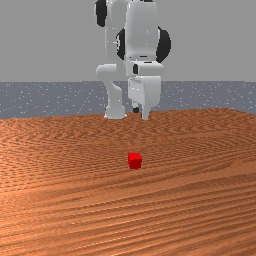
\includegraphics[width=0.118\textwidth]{media/appendix/fs_pick/f0.jpg} &
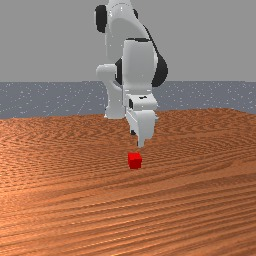
\includegraphics[width=0.118\textwidth]{media/appendix/fs_pick/f1.jpg} &
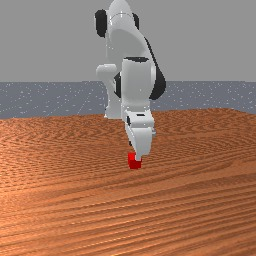
\includegraphics[width=0.118\textwidth]{media/appendix/fs_pick/f2.jpg} &
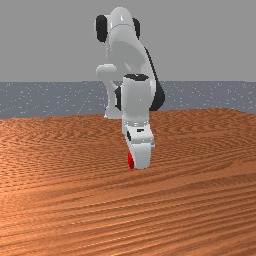
\includegraphics[width=0.118\textwidth]{media/appendix/fs_pick/f3.jpg} &
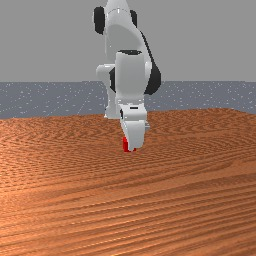
\includegraphics[width=0.118\textwidth]{media/appendix/fs_pick/f4.jpg} &
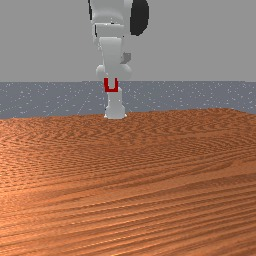
\includegraphics[width=0.118\textwidth]{media/appendix/fs_pick/f5.jpg} &
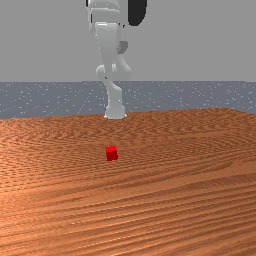
\includegraphics[width=0.118\textwidth]{media/appendix/fs_pick/f6.jpg} &
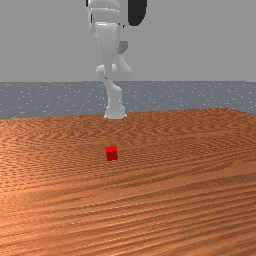
\includegraphics[width=0.118\textwidth]{media/appendix/fs_pick/f7.jpg} \\
\end{tabular}\\[2pt]
{\footnotesize Pick, grasps and lifts then releases.}\par}
\vspace{8pt}
{\centering
\setlength{\tabcolsep}{1pt}\renewcommand{\arraystretch}{0.5}
\begin{tabular}{@{}cccccccc@{}}
{\scriptsize 1} & {\scriptsize 1} & {\scriptsize 1} & {\scriptsize 2} & {\scriptsize 2} & {\scriptsize 2} & {\scriptsize 2} & {\scriptsize 4} \\

\includegraphics[width=0.118\textwidth]{media/appendix/fs_push/f0.jpg} &

\includegraphics[width=0.118\textwidth]{media/appendix/fs_push/f1.jpg} &

\includegraphics[width=0.118\textwidth]{media/appendix/fs_push/f2.jpg} &

\includegraphics[width=0.118\textwidth]{media/appendix/fs_push/f3.jpg} &

\includegraphics[width=0.118\textwidth]{media/appendix/fs_push/f4.jpg} &

\includegraphics[width=0.118\textwidth]{media/appendix/fs_push/f5.jpg} &

\includegraphics[width=0.118\textwidth]{media/appendix/fs_push/f6.jpg} &

\includegraphics[width=0.118\textwidth]{media/appendix/fs_push/f7.jpg} \\
\end{tabular}\\[2pt]
{\footnotesize Push, pushes toward the goal then stalls.}\par}
\vspace{8pt}
{\centering
\setlength{\tabcolsep}{1pt}\renewcommand{\arraystretch}{0.5}
\begin{tabular}{@{}cccccccc@{}}
{\scriptsize 1} & {\scriptsize 1} & {\scriptsize 2} & {\scriptsize 2} & {\scriptsize 3} & {\scriptsize 3} & {\scriptsize 1} & {\scriptsize 1} \\

\includegraphics[width=0.118\textwidth]{media/appendix/fs_stack/f0.jpg} &

\includegraphics[width=0.118\textwidth]{media/appendix/fs_stack/f1.jpg} &

\includegraphics[width=0.118\textwidth]{media/appendix/fs_stack/f2.jpg} &

\includegraphics[width=0.118\textwidth]{media/appendix/fs_stack/f3.jpg} &

\includegraphics[width=0.118\textwidth]{media/appendix/fs_stack/f4.jpg} &

\includegraphics[width=0.118\textwidth]{media/appendix/fs_stack/f5.jpg} &

\includegraphics[width=0.118\textwidth]{media/appendix/fs_stack/f6.jpg} &

\includegraphics[width=0.118\textwidth]{media/appendix/fs_stack/f7.jpg} \\
\end{tabular}\\[2pt]
{\footnotesize Stack, carries the cube then drops it.}\par}
\vspace{8pt}

